\section {Hydration Structure}

To compare the KS-DFT and classical interaction potentials, the O$_{mal}$-H$_{wat}$ radial distribution functions (RDF) are given in Figure \ref{fig:rdf} (where the subscripts ``mal'' refers to one of the malonic acid oxygens, and ``wat'' refers to water hydrogens). Both the KS-DFT (black) and classical (green) interaction potential RDFs are plotted in Figure \ref{fig:rdf}. The two RDFs shown are of the O$_{alcohol}$-H$_{wat}$ (left) and the O$_{carbonyl}$-H$_{wat}$ (right). There is reasonable agreement between the hydration structures calculated using the different interaction potentials. This is an indication that some features of the water packing around the carboxylic acid groups are reproduced in the classical potential in comparison with the KS-DFT interaction potential. Differences between the two interaction potentials appear mostly in the first solvation shell when looking at both the alcohol and carbonyl oxygen RDFs of Figure \ref{fig:rdf}. In the alcohol oxygen plot, the classical potential shows significantly more structure in the first peak, while the trend is reversed in the plot of the double-bonded carbonyl oxygen RDF. This is likely due to the inability of the classical potential to fully reproduce resonance structures of the carboxylic acids. Consequently, this will likely lead to a more symmetric solvation structure than the KS-DFT. The ability of the classical interaction potential to capture the asymmetry of the solvation structure will become more apparent near the water interfacial region. Thus, although the classical potential, which is based on point charges and point polarizabilities, produces a similar average structure, it does not fully capture the resonance structure that is likely very important in the hydrogen bonded states of the malonic acid.

% suggest the deficiency in the classical, and how a better model should be developed to capture that first peak on the alcohol.
\begin{figure}[h!]
	\begin{center}
		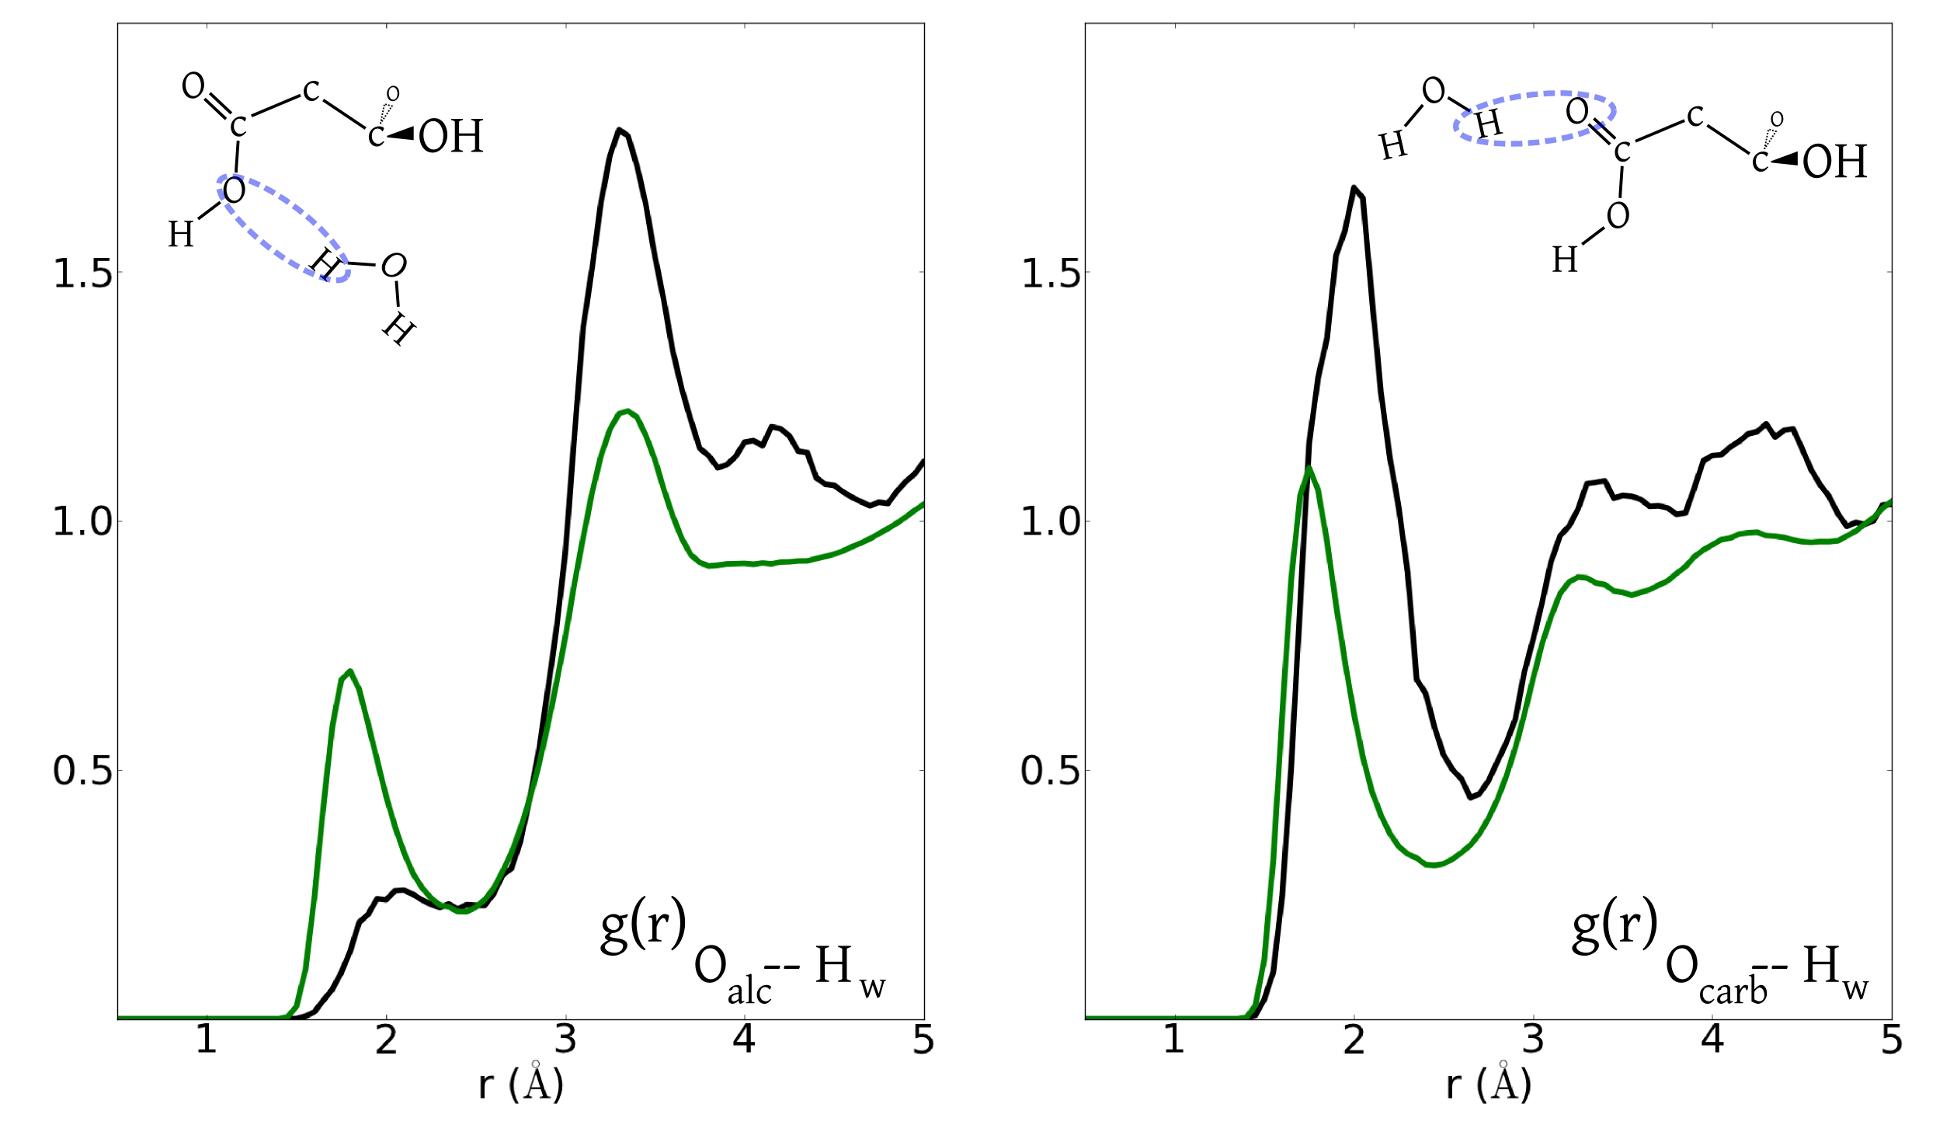
\includegraphics[scale=1.0]{images/rdf/MalonicRDF-small.png}
		\caption{Radial distribution functions, g(r), were calculated for the pair correlations between the acid oxygens and water hydrogen atoms. The acid alcohol moiety oxygen - water hydrogen RDF (left) and the carbonyl oxygen - water hydrogen RDF (right) are plotted. Each RDF is shown for both the KS-DFT simulations of the present study (black), and for classical MD simulations (green) taken from a data set used for a recently published study by our group.\cite{Blower2012}}
		\label{fig:rdf}
	\end{center}
\end{figure}
